\documentclass{article}
\documentclass[a4paper, 11pt]{article} % Font size (can be 10pt, 11pt or 12pt) and paper size (remove a4paper for US letter paper)

\usepackage[protrusion=true,expansion=true]{microtype} % Better typography
\usepackage{graphicx} % Required for including pictures
\usepackage{wrapfig} % Allows in-line images

\usepackage{mathpazo} % Use the Palatino font
\usepackage[T1]{fontenc} % Required for accented characters

\usepackage{graphicx} % Allows including images
\usepackage{booktabs} % Allows the use of \toprule, \midrule and \bottomrule in tables
\usepackage{epstopdf,epsfig}
\usepackage{amsthm}
\usepackage{amsmath}
\usepackage{mathtools}
\usepackage{tikz}
\usepackage{cancel}
\usepackage{comment}
\usepackage[normalem]{ulem}
\usetikzlibrary{arrows, automata, shapes,positioning}
\usepackage{listings}
\lstset{language=Haskell}

\graphicspath{{./}{../img}}

\linespread{1.05} % Change line spacing here, Palatino benefits from a slight increase by default

\makeatletter
\renewcommand\@biblabel[1]{\textbf{#1.}} % Change the square brackets for each bibliography item from '[1]' to '1.'
\renewcommand{\@listI}{\itemsep=0pt} % Reduce the space between items in the itemize and enumerate environments and the bibliography

\renewcommand{\maketitle}{ % Customize the title - do not edit title and author name here, see the TITLE block below
\begin{flushright} % Right align
{\LARGE\@title} % Increase the font size of the title

\vspace{50pt} % Some vertical space between the title and author name

{\large\@author} % Author name
\\\@date % Date

\vspace{40pt} % Some vertical space between the author block and abstract
\end{flushright}
}

%----------------------------------------------------------------------------------------
%	TITLE
%----------------------------------------------------------------------------------------

\title{\textbf{Test and verification}\\ %
% Title
approaches in conformance checking} % Subtitle

\author{\textsc{Kevin Jahns} % Author
\\{\textit{English Communication for Engineers}}} % Institution

\date{\today} % Date

%----------------------------------------------------------------------------------------

\begin{document}

\maketitle % Print the title section

%----------------------------------------------------------------------------------------
%	ABSTRACT AND KEYWORDS
%----------------------------------------------------------------------------------------

\section*{Introduction}
Testing is obligatory for good software development, and not just because it
eases bug finding: Since we use technology everyday (e.g. airplanes and traffic
circulation) it is evident that software bugs can cost lifes. Furthermore
testing is important for the economy: In 2002 a study stated that software errors cost the U.S.
economy $ \$59.5$ billion US-dollars annually, whereat most of this cost could
be avoided by more exhaustive testing \cite{nist}. A recent study which was
initiated by the Cambridge University states that software bugs cost the 
overall economy $ \$ 312 $  billion US-dollars because debugging is inefficient
\cite{cambridge_errors}.
Many software companies still use trivial testing approaches like
\textit{Monkey Testing}. More enhanced testing approaches could safe costs and 
in addition make the software better. Moreover there are approaches to
\textit{verify} that a software does not malfunction. But the crux of testing
and verifying is expressing \textit{conformance}. 

\begin{wrapfigure}{r}{0.4\textwidth} % Inline image example
\caption{Candy machine specification}
\label{candymachine}
\begin{center}
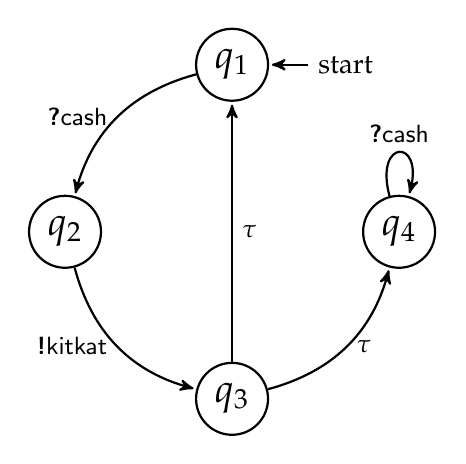
\begin{tikzpicture}[->,>=stealth',shorten >=1pt,auto,node distance=3cm,
                    thick,main
                    node/.style={circle,draw,font=\sffamily\Large\bfseries},
                    %initial text={   }
                    ] 
  \node[initial,initial where=right, main node] (1) [] {$q_1$};
  \node[main node] (2) [below left of=1] {$q_2$};
  \node[main node] (3) [below right of=2] {$q_3$};
  \node[main node] (4) [below right of=1] {$q_4$};

  \path[every node/.style={font=\sffamily\small}]
    (1) edge [bend right] node[left] {{\bfseries ?}cash} (2)
    (2) edge [bend right] node[left] {{\bfseries !}kitkat} (3)
    (3) edge node [right] {$\tau$} (1)
    (4) edge [loop above] node {{\bfseries ?}cash} (4)
    (3) edge [bend right] node[right] {$\tau$} (4);
\end{tikzpicture}
\end{center}
\end{wrapfigure}
\section*{Testing}
Until now most software developers write test cases for software by hand or just
execute the program by themselves. They write test in the form of executable
code. Obviously this is not the state of the art. A more expressive definition
of conformance is via an \textit{Labeled Transition System} (LTS).
In figure \ref{candymachine} we express what a candy machine can do and cannot
do in the form of a specification.
\begin{enumerate}
  \item A candy machine starts in state $q_1$
  \item After the candy machine gets cash it must output a
  kitkat and go into state $q_2$
  \item Then it may either go back into state $q_1$ or it goes to state $q_4$
  \item In state $q_4$ it must not output a kitkat and only accept cash.
\end{enumerate}

\section*{Conformance}
There are various way to express conformance: 
\begin{enumerate}
  \item Statements like ``Never do {\color{red}this}'' are called
  \textit{persistent properties}
  \item State
\end{enumerate}


%------------------------------------------------

\section*{Conclusion}

\bibliographystyle{unsrt}

\bibliography{../sample}

%----------------------------------------------------------------------------------------

\end{document}